\chapter{Applications}
\label{ch:Applications}
\section{Introduction}
The use of the area under the receiver operating curve (AUC) as a measure of performance in SDM is discussed in Section \ref{sec:AUC}. In Section \ref{sec:POData} (resp.\ \ref{sec:PAData}) the performance of the techniques is discussed in the case of presence-only (resp.\ presence-absence) data. In both these sections the models were fit by using a training set and then the AUC values were calculated on a test set. The training set consists of \nicefrac{3}{4}'th of the data while the test set contains the other \nicefrac{1}{4}'th.\\


\section{AUC as a measure of classification performance in SDM}
\label{sec:AUC}
To measure the performance of the classification method the AUC is used. Using the AUC to measure the performance of SDMs has been criticized \parencite{lobo_auc:_2008, jimenez-valverde_insights_2012}. However, most of the issues that are usually raised are not of particular interest in our case. Before studying the AUC values it is interesting to note that there are three main sources of randomness in the calculation of the mean AUC values across the different species. \\ 

First of all, in our set-up we could consider the species that are considered as drawn from a pool of all species in the databases. Of course this assumption is violated since we selected the species conditional on certain characteristics. Hence a more accurate depiction would be to say that the species are a stratified sample from the pool of available species.  \\

Secondly, the parameters in the classifications methods are estimated by using the training set. The elements of the training set can be seen sample of presence, and background or absence points from the corresponding distributions. The predicted probabilities, and the AUC, are therefore also dependent on the sample of points used.\\

Thirdly, the AUC is calculated on the test set which again consists of a sample of random presence, and background or absence points from the corresponding distributions. Thus even if the classifier was fixed we would get different AUC values if we use different test sets. \\

It is well known that the AUC statistic is equivalent to the Mann-Whitney U test statistic \parencite{hanley_meaning_1982}. Therefore the theory surrounding the Mann-Whitney U test statistic can provide us with standard errors (SE), asymptotic distributions, etc. However, these results were derived by assuming that the classifier is fixed. Given that also the training set and the considered species can be seen as a random sample these results are not directly applicable. A rigorous way to inspect the distribution of the AUC values would be to use a bootstrap method to construct e.g.\ confidence intervals. In our situation this is, however, computationally infeasible. In the end we opted to only report standard deviations (SD) and mean values.\\

\section{Presence-only data}
\label{sec:POData}
\subsection{Results}
All the methods described in Chapter \ref{ch:Implementations} were fitted on the GBIF data. A plot of the AUC values can be found in Figure \ref{fig:PrOnlyAUC} and summary measures can be found in Table \ref{tab:PrOnlyAUC}. Few rigorous tests are performed in this section. This because, given the small sample size and the fact that the AUC values are quite close, the power of such tests, using the usual $5\%$ significance level, is very low. Therefore the discussion of the results is rather short and mainly used as a preliminary study to generate interesting research questions for the simulation study of Chapter \ref{chap:SimulationStudy}. \\


\begin{table}[!htb]
\makebox[\textwidth][c]{
\begin{tabular}{lcccccc}
 & \multicolumn{2}{c}{All variables} & \multicolumn{2}{c}{Bioclimatic variables} & \multicolumn{2}{c}{Difference}\\
\cline{2-3} \cline{4-5} \cline{6-7}\\
Method & Mean AUC & SD & Mean AUC & SD & Mean AUC & SD \\
\midrule
Logistic: vanilla               & 0.934 & 0.045 & 0.916 & 0.070 & 0.019    & 0.053 \\
Logistic: backward              & 0.772 & 0.266 & 0.934 & 0.035 & -0.162   & 0.262 \\
Logistic: forward               & 0.661 & 0.242 & 0.599 & 0.277 & 0.062    & 0.330 \\
Logistic: PCA                   & 0.891 & 0.077 & 0.881 & 0.087 & 0.010    & 0.070 \\
Logistic: presence PCA          & 0.838 & 0.172 & 0.887 & 0.090 & -0.049   & 0.101 \\
Logistic: background PCA        & 0.893 & 0.079 & 0.890 & 0.077 & 0.003    & 0.054 \\
Logistic: kernel PCA            & 0.933 & 0.050 & 0.922 & 0.058 & 0.011    & 0.030 \\
Logistic: presence kernel PCA   & 0.947 & 0.033 & 0.927 & 0.052 & 0.020    & 0.040 \\
Logistic: background kernel PCA & 0.937 & 0.048 & 0.935 & 0.039 & 0.002    & 0.028 \\
Logistic: lasso                 & 0.938 & 0.041 & 0.924 & 0.057 & 0.014    & 0.037 \\
Logistic: ridge                 & 0.930 & 0.047 & 0.908 & 0.063 & 0.022    & 0.039 \\
Logistic: select07              & 0.938 & 0.040 & 0.915 & 0.058 & 0.023    & 0.032 \\
GAM: auto selection             & 0.928 & 0.072 & 0.935 & 0.033 & -0.008   & 0.069 \\
GAM: vanilla                    & 0.912 & 0.086 & 0.936 & 0.038 & -0.024   & 0.090 \\
GAM: select07                   & 0.940 & 0.050 & 0.938 & 0.036 & 0.002    & 0.039 \\
MaxEnt                          & 0.921 & 0.055 & 0.932 & 0.041 & -0.011   & 0.028 \\
MaxEnt Vanilla                  & 0.899 & 0.099 & 0.919 & 0.049 & -0.020   & 0.076 \\
ANN                             & 0.946 & 0.046 & 0.948 & 0.032 & -0.003   & 0.040 \\
ANN: vanilla                    & 0.926 & 0.058 & 0.934 & 0.039 & -0.008   & 0.048 \\
GBM                             & 0.958 & 0.032 & 0.944 & 0.033 & 0.014    & 0.030 \\
\bottomrule
\end{tabular}}
\caption{\label{tab:PrOnlyAUC}Summary of the AUC values of the different classifiers fitted on the presence-only data.}
\end{table}

\begin{figure}[!htb]
\center
\makebox[\textwidth][c]{%
	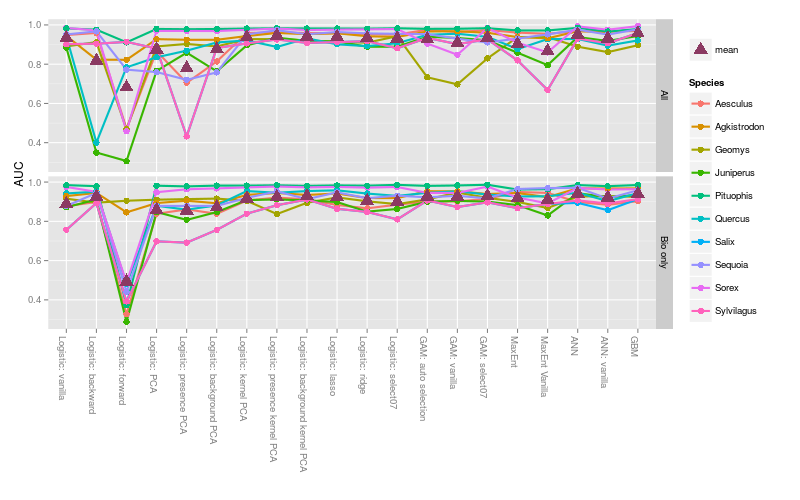
\includegraphics[scale=0.70]{Plots/AUCPlot.png}
}
\caption{\label{fig:PrOnlyAUC}AUC values of the different classifiers fitted on the presence-only data.}
\end{figure}


First of all, it is interesting to note that logistic regression performs quite well. There is a small, non-significant, decrease in mean AUC value when only the bioclimatic variables are considered.\\

The two stepwise selection methods have relatively small mean AUC values and large SDs when all variables are considered. The high SDs indicate that these methods are inherently variable and hence usually lead to unstable predictions. When only the bioclimatic variables are considered the same is true for the forward stepwise selection method, on the other hand backward stepwise selection performs quite well. This could be explained by the fact that the backward selection method becomes a lot more variable when variables with little explanatory power are added. Finally, in comparison with the vanilla logistic regression method the stepwise methods perform quite badly. However, since in the vanilla logistic method only first order terms are considered it might be unfair to say that stepwise selection is inherently worse and a comparison with a logistic regression model with the same polynomial expansion might have been more appropriate. \\ 


The MaxEnt implementation with the default settings performs worse than the implementation in which the penalization parameter is selected by CV. Although MaxEnt is very popular in SDM applications it does not seem to perform better than simpler models as logistic regression. Even though our small sample size does not allow us to dispute the popularity of MaxEnt our results seem to show that even if there is a gain in performance over e.g.\ logistic regression it is likely quite small and one might wonder if the loss of interpretability and increased computational cost is worth a small gain in performance. Furthermore, it seems that in most applications of SDM the default value of the penalization parameter is used while our results seem to show that using CV leads to some improvements. \\

GBMs and ANNs seem to consistently lead to high AUC values with low standard deviations. Although these methods are sometimes used in practice they are far less popular than the MaxEnt method. Given our results it seems like MaxEnt might be overused and it seems appropriate to at least consider some other machine learning methods when building SDM. \\ 

None of the PCA logistic regression methods seem to perform well, i.e.\ the mean AUC is lower than the mean AUC of logistic regression and the SDs are quite large. Both when only the bioclimatic variables and when all variables are used at least one of the KPCA logistic regression methods tends to outperform the logistic regression model. At first glance there does not seem to be a systematic difference between using the presence or the background observations in the (K)PCA methods. To rigorously test this two Wilcoxon signed-rank tests were performed. The p-value corresponding with the test for the PCA (resp.\ KPCA) method is $0.32$ (resp.\ $0.11$) and hence the null-hypothesis of no difference between the methods is accepted. \\

The three version of GAMs that we consider all seem to perform better than logistic regression when only the bioclimatic variables are considered. When all variables are considered the select07 variable selection method in combination with a GAM still performs decently while the two other methods seem to deteriorate slightly.  \\

The penalized logistic regression models perform approximately on par with the standard logistic regression model. Finally, the logistic regression model combined with the select07 rule seems to slightly outperform the standard logistic regression model when bioclimatic variables are considered and on par when all variables are used. \\

To test whether or not using only the bioclimatic variables has a profound effect a Wilcoxon signed-rank test was performed for each method. These tests are of interest because on one hand they provide information on the usefulness of non-bioclimatic variables, i.e. is there an increase in classification performance. Also a decrease of the AUC values is of interest, it could namely be interpreted as adding irrelevant predictors which lead to over-fitting. Even before performing a multiple testing correction none of the tests were significant at the $5$\% level. It is therefore concluded that in this limited study there is no statistically significant difference between using only the bioclimatic variables or all variables. 

\section{Presence-absence data}
\label{sec:PAData}
In this section the classification methods are used in combination with the FIA presence-absence data. First of all, although a variation of the MaxEnt method can be used for presence-absence data this is nearly never done. Furthermore, instead of fitting three different variations of (K)PCA logistic regression it was decided to only use the standard approach. This was done to speed up the computations, and unlike in the presence-only scenario the absence points are ``real'' observations. Since only five species were considered there are no statistically significant results in this section. The inspection is mainly done to make sure that the different methods show approximately the same performance characteristics for both presence-only and presence-absence data. The results can be found in Section \ref{sec:PAResults}. Finally, because there are at between $42029$ and $287860$ plot locations available the fitting of the models leads to computational problems. A solution to these problems is proposed in Section \ref{sec:CaseControlSubsampling}.
\subsection{Case-control sampling}
\label{sec:CaseControlSubsampling}
Because of computational considerations it was decided to use a subset of the presence-absence data to fit the models upon. More particularly, the subsample consists of all the presence points and $5000$ randomly sampled absence points. This is a form of case-control sampling and the effect of doing this has been studied \parencite{king_logistic_2001}. \\

In the case of logistic regression some algebra along the lines of Equation \ref{eq:IPPSampling} shows that only the intercept is affected by the sub-sampling \parencite{king_logistic_2001}. Although the underlying coefficients stay the same the variance of the estimators increases slightly. Because we only subsample the absence points this increase should be somewhat limited. Intuitively it makes sense that a rare presence point contains more information about the coefficients than one of the abundant absence points. In the case of logistic regression this can rigorously be deduced by observing that a term of the form $P(Y=1|\bm{X} = \bm{x}) \left[1- P(Y=1|\bm{X} = \bm{x}) \right]$ turns up in the variance expression. Usually this term is quite a lot smaller for the abundant cases and hence leaving some out does not lead to a huge increase of the variance. \\ 

Although the previous paragraph focusses on logistic regression the same reasoning can be applied to the other methods considered. Finally, in the last two decades there has been quite some research on issues related to imbalanced data-sets and perhaps more efficient ways of dealing with the imbalance exist, see e.g.\ \cite{chawla2005data} for an overview of other methods. \\

\subsection{results}
\label{sec:PAResults}
The mean and and the standard deviations can be found in Table \ref{tab:PrAbAUC} and Figure \ref{fig:PrAbAUC} shows a plot of the estimated AUC values. \\

\begin{table}[!htb]
\makebox[\textwidth][c]{
\begin{tabular}{lcccccc}
 & \multicolumn{2}{c}{All variables} & \multicolumn{2}{c}{Bioclimatic variables} & \multicolumn{2}{c}{Difference}\\
\cline{2-3} \cline{4-5} \cline{6-7}\\
Method & Mean AUC & SD & Mean AUC & SD & Mean AUC & SD \\
\midrule
Logistic: vanilla    & 0.961 & 0.027 & 0.951 & 0.041 & 0.010   & 0.022 \\
Logistic: backward   & 0.682 & 0.301 & 0.703 & 0.276 & -0.021  & 0.355 \\
Logistic: forward    & 0.774 & 0.284 & 0.660 & 0.333 & 0.115   & 0.208 \\
Logistic: PCA        & 0.913 & 0.084 & 0.926 & 0.063 & -0.013  & 0.055 \\
Logistic: kernel PCA & 0.950 & 0.052 & 0.922 & 0.086 & 0.028   & 0.041 \\
Logistic: lasso      & 0.960 & 0.042 & 0.968 & 0.022 & -0.008  & 0.025 \\
Logistic: ridge      & 0.957 & 0.044 & 0.948 & 0.049 & 0.009   & 0.016 \\
Logistic: select07   & 0.756 & 0.239 & 0.859 & 0.206 & -0.102  & 0.219 \\
GAM: auto selection  & 0.925 & 0.098 & 0.954 & 0.038 & -0.029  & 0.062 \\
GAM: vanilla         & 0.877 & 0.117 & 0.927 & 0.074 & -0.049  & 0.098 \\
GAM: select07        & 0.948 & 0.062 & 0.954 & 0.052 & -0.006  & 0.019 \\
ANN                  & 0.973 & 0.020 & 0.971 & 0.024 & 0.002   & 0.007 \\
ANN: vanilla         & 0.962 & 0.036 & 0.963 & 0.035 & -0.001  & 0.009 \\
GBM                  & 0.977 & 0.014 & 0.961 & 0.030 & 0.016   & 0.023 \\
\bottomrule
\end{tabular}}
\caption{\label{tab:PrAbAUC}Summary of the AUC values of the different classifiers fitted on the presence-absence data.}
\end{table}


\begin{figure}[!htb]
\center
\makebox[\textwidth][c]{%
	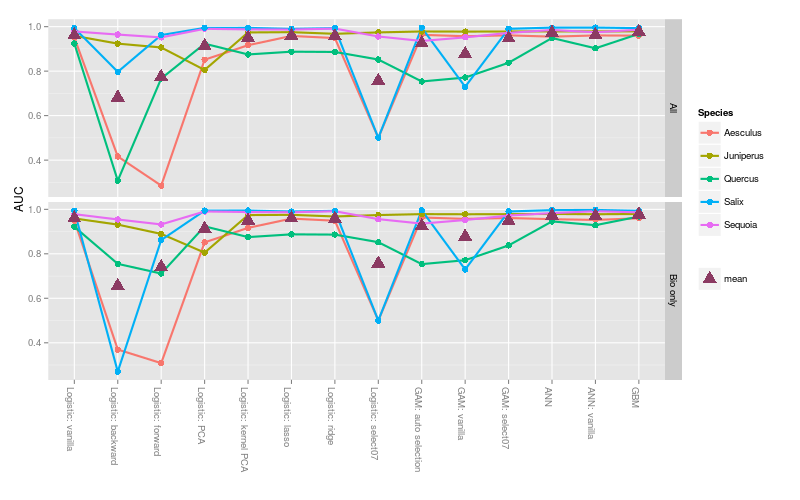
\includegraphics[scale=0.70]{Plots/AUCPAPlot.png}
}
\caption{\label{fig:PrAbAUC}AUC values of the different classifiers fitted on the presence-absence data.}
\end{figure}

The methods tend to show the same characteristics as observed in Section \ref{sec:PAResults}, hence we only quickly review the main points. \\


It is readily seen that the logistic regression model performs quite well, i.e.\ it leads to relatively high average AUC values and its SD is quite low. The stepwise methods both have large SD and have the lowest average AUC values. The GBM and ANN methods are the two methods with the largest average AUC and both have relatively small SD. The two penalized regression methods seem to perform on par with the standard logistic regression implementation. Preprocessing the data by using PCA before performing logistic regression seems to lead to a small decrease in performance. Doing the same but with the non-linear KPCA method leads to results comparable with those of standard logistic regression. \\

The only deviation from the presence-only scenario is the logistic07 method. When this method is used with the presence-absence data it is quite variable and leads to low average AUC values. \\

Finally, there seems to be no specific trend, relative to the SEs, when the models are fitted on all versus only the bioclimatic variables. 




